\documentclass[lang=cn,11pt,a4paper,cite=authornum]{paper}

\title{操作系统 实验二:进程控制 \\ 实验报告}
\author{毛子恒 \\ 2019211397}
\institute{北京邮电大学\ 计算机学院}

\date{\zhtoday}

% 本文档命令
\nocite{*}

\begin{document}

\maketitle

\section{概览}

\subsection{实验内容}

\subsubsection{实验内容一}

Collatz猜想:任意写出一个正整数$N$,并且按照以下的规律进行变换:

\begin{itemize}
    \item 如果是个奇数,则下一步变成$3N+1$;
    \item 如果是个偶数,则下一步变成$N/2$。
\end{itemize}

无论$N$是怎样的一个数字,最终都会变成1。

采用系统调用\mintinline{C}{fork()},编写一个C程序,以便在子进程中生成这个序列。要求:

\begin{enumerate}
    \item 从命令行提供启动数字。
    \item 由子进程输出数字序列。
    \item 父进程等子进程结束后再退出。
\end{enumerate}

\subsubsection{实验内容二}

以共享内存技术编程实现Collatz猜想。

要求在父子进程之间建立一个共享内存对象,允许子进程将序列内容写入共享内存对象,当子进程完成时,父进程输出序列。

父进程包括如下步骤:

\begin{enumerate}
    \item 建立共享内存对象(\mintinline{C}{shm_open()},\mintinline{C}{ftruncate()},\mintinline{C}{mmap()})
    \item 建立子进程并等待他终止。
    \item 输出共享内存的内容。
    \item 删除共享内存对象。
\end{enumerate}

\subsubsection{实验内容三}

设计一个程序,通过普通管道进行通信,让一个进程发送一个字符串消息给第二个进程,第二个进程收到此消息后,变更字母的大小写,然后再发送给第一个进程。比如,第一个进程发消息:“I am Here”,第二个进程收到后,将它改变为:“i AM hERE”之后,再发给第一个进程。

\subsection{实验环境}

\begin{itemize}
    \item openEuler 20.03 64bit with ARM
    \item gcc version 7.3.0
    \item vim 8.1
\end{itemize}

\section{实验设计}

\subsection{实验内容一}

\subsubsection{相关API}

\begin{itemize}
    \item \mintinline{C}{pid_t fork(void);}:创建子进程,子进程是调用该函数的进程的拷贝。子进程与父进程有各自单独的地址空间,在调用之后其中的内容是相同的。如果创建成功,该函数返回给父进程以子进程的PID,给子进程返回0。
    \item \mintinline{C}{pid_t wait(int *wstatus);}:暂停调用该函数的进程直到所有子进程都终止,当成功时,返回终止的子进程的PID,失败时返回-1。 
\end{itemize}

\subsubsection{设计概述}

如\figref{fig:UML1}所示,父进程首先通过标准输入读取$n$,之后通过\mintinline{C}{fork()}函数创建子进程,并调用\mintinline{C}{wait()}函数等待子进程结束。

子进程得到与父进程数据段地址空间的一份副本,其中包含$n$的值。之后子进程通过循环计算序列并且输出,之后通过\mintinline{C}{return 0}终止。

父进程回收子进程后,输出一行字符串之后终止。

\begin{figure}[htbp]

    \centering
    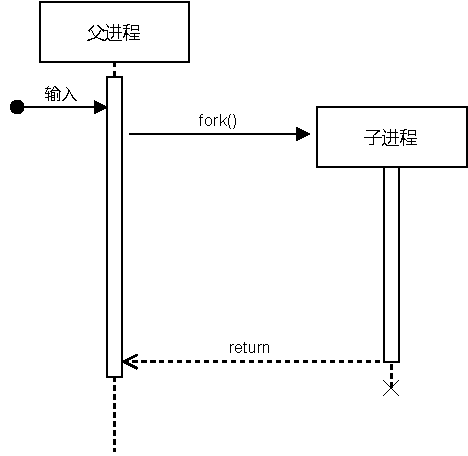
\includegraphics[width=0.6\linewidth]{./images/UML1.pdf}
    \caption{实验内容一时序图\label{fig:UML1}}

\end{figure}

\subsection{实验内容二}

\subsubsection{相关API}

\begin{itemize}
    \item \mintinline{C}{int shm_open(const char *name, int oflag, mode_t mode);}:打开(或者创建新的同时打开)一个POSIX共享内存对象。共享内存对象可以作为一个句柄提供给另一个进程来访问一块共享内存。\mintinline{C}{text}参数用于指定一个共享内存对象的名字,推荐格式为\mintinline{text}{/somename};\mintinline{text}{oflag}用于指定一些选项,例如\mintinline{text}{O_RDONLY}表示对象只读,\mintinline{text}{O_RDWR}表示对象可读可写,\mintinline{text}{O_CREAT}表示如果对象不存在则创建一个新对象,新对象的权限通过\mintinline{text}{mode}参数设置。如果成功,该函数返回一个文件描述符(一个非负整数)。
    \item \mintinline{C}{int ftruncate(int fd, off_t length);}:通过该函数给文件(即之前创建的共享内存对象)分配空间,\mintinline{text}{fd}表示文件描述符,\mintinline{text}{length}为裁切的长度。如果成功,返回0.
    \item \mintinline{C}{void *mmap(void *addr, size_t length, int prot, int flags, int fd, off_t offset);}:在当前进程的虚拟地址空间中创建一个映射,\mintinline{text}{addr}指明映射的起始地址,若为\mintinline{text}{NULL},则内核自动选择一个页对齐的地址创建映射;\mintinline{text}{length}指明映射的长度;\mintinline{text}{prot}指明对映射的内存保护选项,包括\mintinline{text}{PROT_EXEC}可执行、\mintinline{text}{PROT_READ}可读、\mintinline{text}{PROT_WRITE}可写、\mintinline{text}{PROT_NONE}不可访问;\mintinline{text}{flags}决定对映射的修改是否对其他进程可见,并且修改是否会被代入到构成映射的文件,\mintinline{text}{MAP_SHARED}表示对该映射的修改会分享给其他进程;\mintinline{text}{fd}为文件描述符;\mintinline{text}{offset}为文件中起始位置的偏移量。当映射成功时,该函数返回一个指向映射区域的指针。
    \item \mintinline{C}{int munmap(void *addr, size_t length);}:删除给定地址的映射,之后对于给定地址的引用会无效。当进程终止时,映射也会被自动删除。
    \item \mintinline{C}{int shm_unlink(const char *name);}:移除一个共享内存对象名称,如果所有的进程都已经删除了对该对象的映射,那么该内存区域会被释放。
\end{itemize}

\subsubsection{设计概述}

流程仍然如\figref{fig:UML1}所示,父进程首先读取$n$,创建共享内存对象并且分配空间,创建对共享内存的映射,之后通过\mintinline{C}{fork()}函数创建子进程,并调用\mintinline{C}{wait()}函数等待子进程结束。

子进程得到了$n$和共享内存的地址,计算循环计算序列并且以字符串的形式打印到共享内存中,之后删除映射并通过\mintinline{C}{return 0}终止。

父进程回收子进程后,向标准输出打印共享内存中的字符串,之后删除映射并且移除共享内存对象(此时会释放共享内存),最后终止。

\subsection{实验内容三}

\subsubsection{相关API}

\begin{itemize}
    \item \mintinline{C}{int pipe(int pipefd[2]);}:创建一个单向的管道,\mintinline{text}{pipefd}用于返回管道两端的文件描述符,分别为读取端和写入端。如果成功,函数返回0。
    \item \mintinline{C}{int close(int fd);}:关闭一个文件描述符。
    \item \mintinline{C}{ssize_t write(int fd, const void *buf, size_t count);}:向文件描述符\mintinline{C}{fd}指明的文件写入从\mintinline{text}{buf}开始的\mintinline{text}{count}个字节。若成功,返回写入的字节数。
    \item \mintinline{C}{ssize_t read(int fd, void *buf, size_t count);}:从文件描述符\mintinline{C}{fd}指明的文件读取到从\mintinline{text}{buf}开始的缓冲区,最多读取\mintinline{text}{count}个字节。若成功,返回读取的字节数。
\end{itemize}

\subsubsection{设计概述}

如\figref{fig:UML2}所示,父进程首先创建两个管道,之后通过\mintinline{C}{fork()}函数创建子进程。

子进程得到与父进程数据段地址空间的一份副本,包含两个管道的入口和出口描述符。子进程首先关闭上行(子进程到父进程)管道的读取端和下行(父进程到子进程)管道的写入端,之后子进程调用\mintinline{C}{read()}函数阻塞,等待下行管道的输入。

父进程首先关闭上行管道的写入端和下行管道的读取端,之后从标准输入中读入一行字符串,并且写入到下行管道,之后调用\mintinline{C}{read()}函数阻塞,等待上行管道的输入。

子进程得到下行管道的输入后,对字符串进行大小写转换,之后写入到上行管道,并且关闭剩余的文件描述符并终止。

父进程得到上行管道的输入后,向标准输出打印字符串,关闭剩余的文件描述符并终止。

\begin{figure}[htbp]

    \centering
    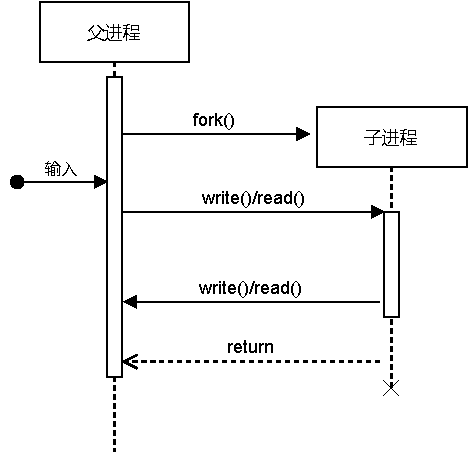
\includegraphics[width=0.6\linewidth]{./images/UML2.pdf}
    \caption{实验内容三时序图\label{fig:UML2}}

\end{figure}

\section{运行结果及分析}

\subsection{实验内容一}

\subsubsection{输入}

\begin{code}
\begin{minted}{text}
35
\end{minted}
\end{code}

\subsubsection{输出}

\begin{code}
\begin{minted}{text}
35 106 53 160 80 40 20 10 5 16 8 4 2 1
Done.
\end{minted}
\end{code}

\subsubsection{分析}

主进程成功创建了子进程,子进程计算并输出了序列。

\subsection{实验内容二}

输入和输出与实验内容一相同,略。

\subsubsection{分析}

主进程成功创建了共享内存和子进程,子进程计算了序列并且输出到共享内存,主进程打印了共享内存的内容。

\subsection{实验内容三}

\subsubsection{输入}

\begin{code}
\begin{minted}{text}
I am Here
\end{minted}
\end{code}

\subsubsection{输出}

\begin{code}
\begin{minted}{text}
i AM hERE
\end{minted}
\end{code}

\subsubsection{分析}

主进程和子进程之间成功用管道交换信息。

\section{实验总结}

本次实验中我利用POSIX API编写了三个与进程控制和通信有关的程序,使我对相关知识点的掌握更加牢固。

我通过查阅\href{https://man7.org/linux/man-pages/index.html}{Linux man page}获取相关API的信息,并且参考教材的内容编写程序,编写过程中除了头文件和链接选项没有遇到太多问题。在阅读man page和相关文档的过程中我对进程控制和共享内存模型的有了更多的认识。

本次实验使我的C编程能力和英文文献阅读能力得到提高,我从中收获颇丰。

\end{document}